\chapter{Implementation}

\section{Introduction}

\paragraph{}In order to be able to control the Baxter robot, a ROS environment has to be installed and configured on Ubuntu\footnote{\url{http://sdk.rethinkrobotics.com/wiki/Workstation_Setup}}. The Ubuntu Operating System is run on a virtual machine using the VMWare software. To test the inverse kinematics calculations described in Chapter \ref{chap:inv kin} without the physical Baxter robot, the Gazebo simulator software is used locally on the virtual machine. When the Python code for the inverse kinematics is validated on the simulator, the same code can be tested on the physical robot. 

\section{Python code}
\paragraph{}The code is written in Python programming language using rospy module\footnote{\url{https://github.com/ros/ros_comm}} and the baxter interface\footnote{\url{https://github.com/RethinkRobotics/baxter_interface}} to control the different parts of the robot. The code is made of the two following classes. 

\subsection{BaxterTask class}
\paragraph{}The first one is the BaxterTask class that represents the task that the robot has to accomplish. To define the parameters of the task, a JSON file must be provided to the class containing everything needed such as the positions the robot arm must reach or the speed at which the robot must move. At initialisation of the task, all the points found in the JSON file are converted to joint angles using the inverse kinematics method explained in Chapter~\ref{chap:inv kin}. The method \lstinline[language=Python, style=pythonColor]{inverse_kinematics} is in charge of this conversion. After the calculation of each point, the method \lstinline[language=Python, style=pythonColor]{check_angle_limits} verifies that the angular positions asked by the inverse kinematics are physically feasible. If a value doesn't meet the requirements, a message is sent as a log with the mismatch value.

\subsection{BaxterRobot class}
\paragraph{}The other class is the BaxterRobot class which manages all the communications with the robot. This class also acts as a state machine containing the following states.

\paragraph{Gripper state}The robot is waiting for the operator to put the brush inside the gripper. In this state, each wheel on each arm controls the opening and closing of the gripper of the corresponding arm. With this functionality, the operator can adjust as he wants the orientation of the paintbrush. When ready, the operator can push the button below the wheel on any arm to make the robot enter the next state.

\begin{figure}[!ht]
	\centering
	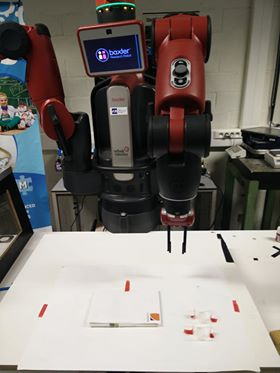
\includegraphics[scale = 0.38]{report/Images/WaitingBrush.jpg}
    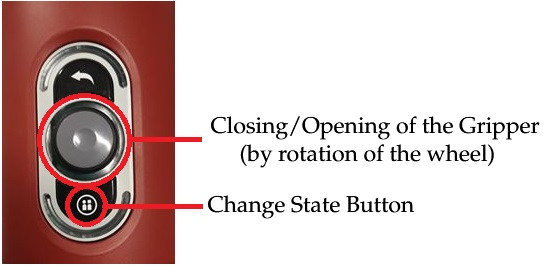
\includegraphics[width = 0.7\textwidth]{report/Images/ArmButtons.jpg}
    \caption{Baxter waiting for the paint brush in gripper state}
    \label{fig:buttons}
\end{figure}

\paragraph{Calibration state}The robot is pointing at a precise location with his arms to allow the operator to check if the working area is at the desired position for the robot. The use of the 2 arms is recommended here as it allows to calibrate the translation and the rotation of the working area (One arm can also be used for calibrating the orientation by pointing at two separated points). When everything is ready, the operator can again push the "change state" button.

\begin{figure}[!ht]
	\centering
	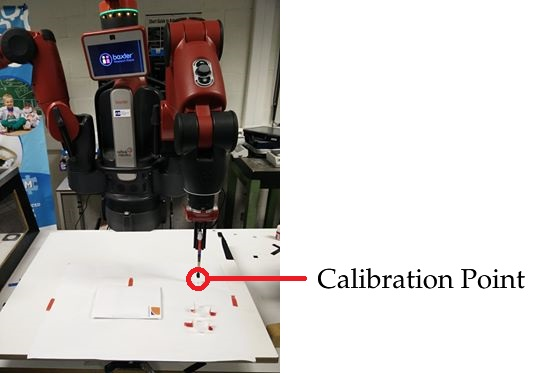
\includegraphics[width = 0.7\textwidth]{report/Images/Calibration.jpg}
    \caption{Baxter pointing the calibration point in calibration state}
    \label{fig:calibration}
\end{figure}

\paragraph{Working state}The robot is now ready to perform the task and reaches successively every position specified in the JSON file.

\begin{figure}[!ht]
	\centering
	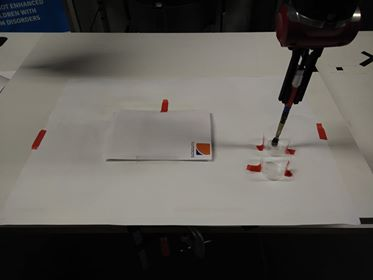
\includegraphics[width = 0.45\textwidth]{report/Images/BaxterPaint.jpg}
	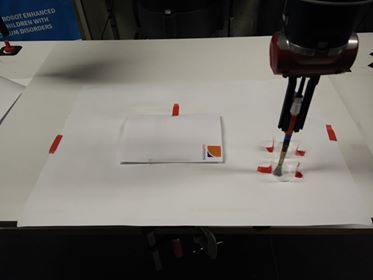
\includegraphics[width = 0.45\textwidth]{report/Images/BaxterWater.jpg}
    \caption{Baxter putting the brush in the paint (left) and in the water (right)}
    \label{fig:PaintWater}
\end{figure}

\subsection{Main function}
\paragraph{}The main function boils down to the creation of an instance of each of the previously mentioned classes and the call of the \lstinline[language=Python, style=pythonColor]{execute} method from the BaxterTask class.

\vspace{2.5cm}

\section{Problems encountered and solutions}
Some problems have been encountered during the project.\\
First the x-axis was oriented at 45$^\circ$ compared to the robot (looking direction) so that an offset (positive for the right arm and negative for the left arm) had to be added to have a more convenient orientation for the application. \\ However, because of the more strict limits of the workspace due to the constraint on the different joints, it was difficult not to reach the limits of its range. Therefore, the point of reference (used for calibration) had to be adjusted to be at a good position.
% The orientation of the other axis of the two arms had also to be verified: both y-axis are pointing to the right and both z-axis are pointing to the bottom.\\
%Another problem using this robot is the limit of the task and joint space of Baxter.

\newpage

\section{Result}
The drawing is shown in Figure \ref{fig:draw}. The result is not too bad, but there is definitely some place for improvement. 

 \begin{figure}[!ht]
	\centering
    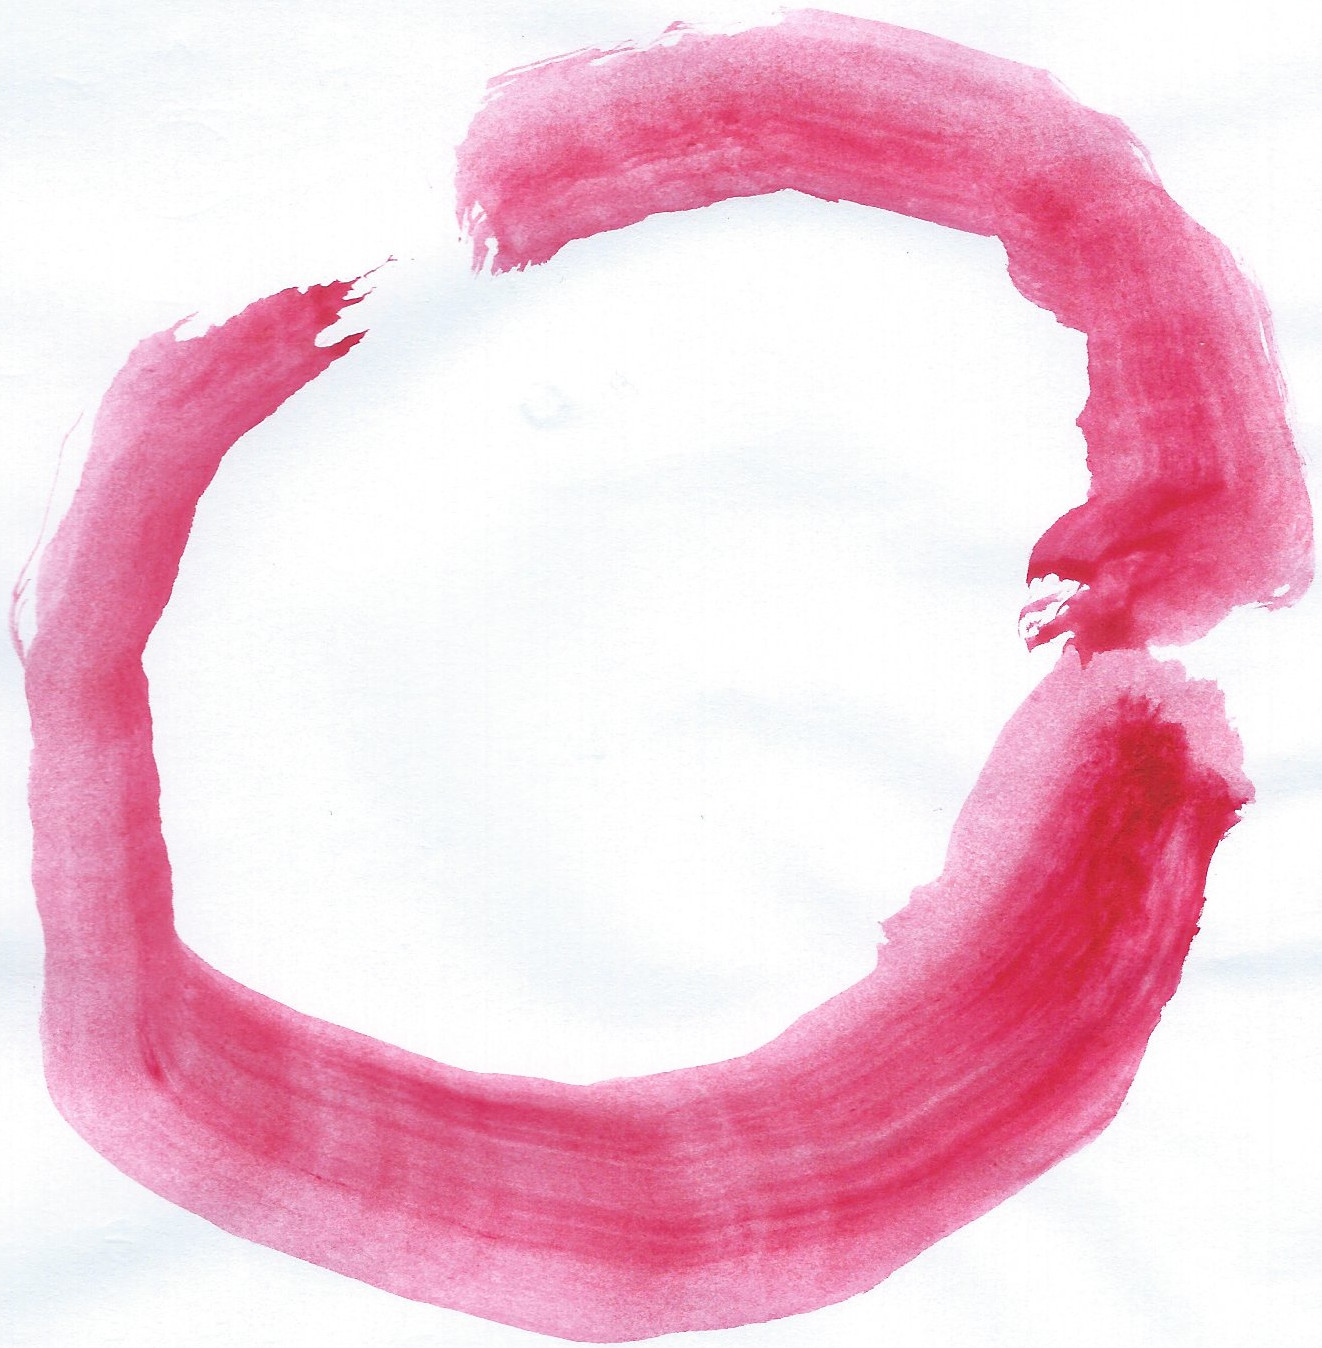
\includegraphics[width = 0.7\textwidth]{Images/masterpiece-cropped.jpg}
    \caption{Final drawing of the robot}
    \label{fig:draw}
\end{figure}

\noindent A first observation is that the thickness of the line varies, which is mainly due to differences in height (but also to brush hair orientation and the amount of paint).\\
\noindent Also, the paintbrush adds some length to the robot arm, which decreases the precision (small angular disturbances of the last joint will have a bigger effect on the precision). It would thus be more convenient to draw a circle with a larger diameter respecting the workspace limits, so as to obtain a better relative precision.\\
\noindent Lastly, it can be seen that the brush lost contact with the paper sheet during a transition (upper-left side of the circle) so that the circle is not closed. This brush elevation can not be avoided using such a position control method, except by increasing the waypoints density. Indeed, the transition control between the discrete successive positions is done by the robot, and can therefore have an inappropriate dynamic behaviour in some applications like precise drawing.\\

\noindent A short video demonstration can be visualized on Youtube: \\\url{https://www.youtube.com/watch?v=0B4mPrNSfEQ}